%!TEX encoding = UTF-8 Unicode

\section{Experimental Results}

We present two types of results: prediction over the effects of actions, and prediction over the word descriptions. In the latter case, we compare the words obtained by the \acl{BN} in the presence of an action prior, with the ones obtained in the absence of the action information.

\subsection{Effect Prediction}

We predict the values of effect-related nodes~(Object Velocity and relative Object--Hand Velocity), given the action node~(provided by the hard decision of Gesture \acp{HMM} when classifying SHOW FIG) and nodes related to object features~(Shape and Size).

TODO expand:
\begin{verbatim}
  p(ObjVel, ObjHandVel | A=tap, F=circle small)

  =

      0.0478    0.0000    0.0000
      0.2921    0.1266    0.0098
      0.0001    0.0903    0.4332
\end{verbatim}
\ie medium or fast motion.

\begin{verbatim}
  p(ObjVel, ObjHandVel | A=tap, F=box big)

  =

      0.9984    0.0002    0.0002
      0.0005    0.0002    0.0000
      0.0000    0.0001    0.0003
\end{verbatim}
\ie slow or no motion.

\subsection{Prediction of Words}

We compare the probability of word occurrence in two situations:
\begin{enumerate}
\item when the robot prior knowledge~(evidence in the \ac{BN}) includes information about object features and effects only, in particular \emph{Color=yellow, Size=big, Shape=circle, ObjVel=fast};

\item when the robot prior knowledge includes, in addition to the above, evidence about the action as observed from the Gestures \acp{HMM}, in particular \emph{Action=tap}.
\end{enumerate}

\begin{figure}
\centering
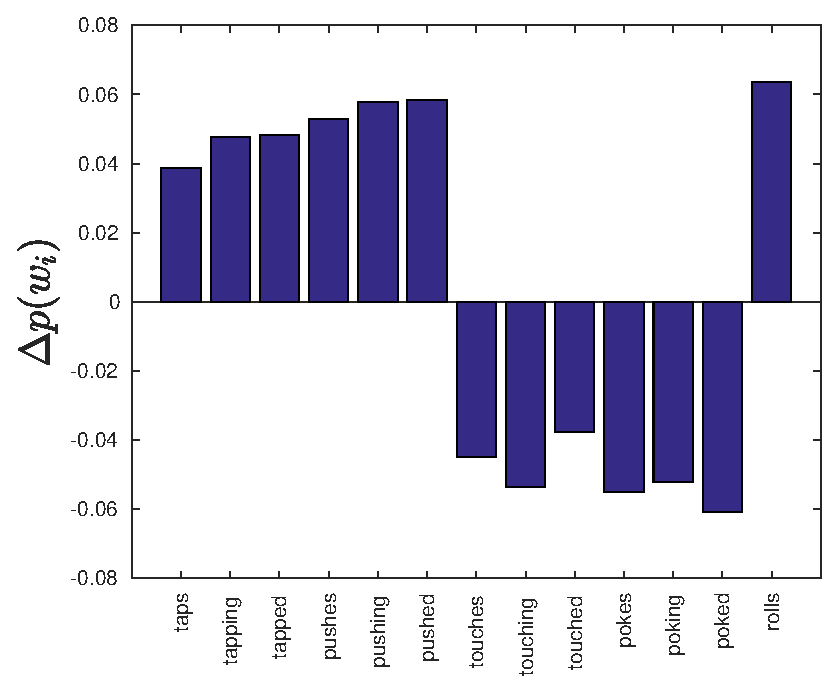
\includegraphics[width=0.9\columnwidth]{partialfig.eps}
\caption{Variation of word occurrence probabilities when we add the tap action evidence~(obtained from the Gesture \acp{HMM}) to the initial evidence about object features and effects.}
\label{fig:probdiff}
\end{figure}

Fig.~\ref{fig:probdiff} shows the variation in word occurrence probabilities between the two cases. We can interpret the difference in the predictions as follows:
\begin{itemize}
\item the probabilities of words related to tapping and pushing increase when a tapping action evidence from the Gestures \acp{HMM} is introduced; conversely, the probabilities of other action words~(touching and poking) decreases;

\item interestingly, the probability of the word \emph{rolling}~(which is an effect of an action onto an oject) also increases when the tapping action evidence is entered. Even though the initial evidence of case~$1$ already included some effect information, it is only now, when the robot perceives that the physical action was a tap, that the event rolling is associated.
\end{itemize}

%We compare the \ac{BN} predictive power in terms of word nodes, with and without the Action prior information provided by the Gesture \acp{HMM}. In other words, we compare~$p(W \mid A, E, F)$ with~$p(W \mid E, F)$.

%TODO work in progress, looking for a combination of E,F which makes the result significant
